\documentclass[11pt,twoside]{scrartcl}
%\documentclass[11pt,twoside]{article}

%opening
\newcommand{\lecid}{15-316}
\newcommand{\leccourse}{Software Foundations of Security and Privacy}
\newcommand{\lecdate}{} %e.g. {October 21, 2013}
\newcommand{\lecnum}{11}
\newcommand{\lectitle}{Truste Computing}
\newcommand{\lecturer}{Matt Fredrikson}
\newcommand{\lecurl}{https://15316-cmu.github.io/index}

\usepackage{varwidth}
\usepackage{lecnotes}
\usepackage[irlabel]{bugcatch}

\usepackage{tikz}
\usetikzlibrary{automata,shapes,positioning,matrix,shapes.callouts,decorations.text,patterns,decorations.pathreplacing,matrix,arrows,chains,calc,tikzmark,petri,topaths}
\pgfdeclarelayer{background}
\pgfdeclarelayer{foreground}
\pgfsetlayers{background,main,foreground}

\usepackage{tkz-berge}
\usepackage[position=bottom]{subfig}

\newcommand{\mx}[1]{\mathbf{\bm{#1}}} % Matrix command
\newcommand{\vc}[1]{\mathbf{\bm{#1}}} % Vector command

% \usepackage[bracketinterpret,seqinfers,sidenotecalculus]{logic}
% \newcommand{\I}{\interpretation[const=I]}

% \newcommand{\bebecomes}{\mathrel{::=}}
% \newcommand{\alternative}{~|~}
% \newcommand{\asfml}{F}
% \newcommand{\bsfml}{G}
% \newcommand{\cusfml}{C}
% \def\sqsubseteqftrule{L}%
% \def\rightrule{R}%

\begin{document}

\newcommand{\atrace}{\omega}%
%% the standard interpretation naming conventions
\newcommand{\stdI}{\dTLint[state=\omega]}%
\newcommand{\Ip}{\dTLint[trace=\atrace]}%
\newcommand{\ws}{\omega}\newcommand{\wt}{\nu}% 

\newcommand{\aff}[2]{\ensuremath{#1~\keywordfont{aff}~#2}}
\newcommand{\ownsr}{\ensuremath{\keywordfont{owns}}}
\newcommand{\isfac}{\ensuremath{\keywordfont{isFaculty}}}
\newcommand{\studof}{\ensuremath{\keywordfont{studentOf}}}
\newcommand{\canopen}{\ensuremath{\keywordfont{canOpen}}}
\newcommand{\matt}{\ensuremath{\mathsf{mfredrik}}\xspace}
\newcommand{\tli}{\ensuremath{\mathsf{tli2}}\xspace}
\newcommand{\admin}{\ensuremath{\mathsf{admin}}\xspace}
\newcommand{\jan}{\ensuremath{\mathsf{janh}}\xspace}
\newcommand{\frank}{\ensuremath{\mathsf{fp}}\xspace}
\newcommand{\office}{\ensuremath{\mathsf{cic2126}}\xspace}
\newcommand{\eduroam}{\ensuremath{\mathsf{er}}\xspace}
\newcommand{\cmu}{\ensuremath{\mathsf{cmu}}\xspace}
\newcommand{\ca}{\ensuremath{\mathsf{ca}}\xspace}
\newcommand{\tca}{\ensuremath{\mathsf{TrustedCA}}\xspace}
\newcommand{\dca}{\ensuremath{\mathsf{DiscountCA}}\xspace}
\newcommand{\tpm}{\ensuremath{\mathsf{tpm}}\xspace}
\newcommand{\pcr}{\ensuremath{\mathsf{PCR}}\xspace}
\newcommand{\store}{\ensuremath{\mathsf{store}}\xspace}
\newcommand{\os}{\ensuremath{\mathsf{os}}\xspace}
\newcommand{\sktpm}{\sk{\tpm}}
\newcommand{\pktpm}{\pk{\tpm}}
\newcommand{\skca}{\sk{\ca}}
\newcommand{\pkca}{\pk{\ca}}
\newcommand{\isstu}{\ensuremath{\keywordfont{isStudent}}\xspace}
\newcommand{\canacc}{\ensuremath{\keywordfont{canAccess}}\xspace}

\newcommand{\pk}[1]{\ensuremath{\keywordfont{pk}_{#1}}\xspace}
\newcommand{\sk}[1]{\ensuremath{\keywordfont{sk}_{#1}}\xspace}
\newcommand{\isca}[1]{\ensuremath{\keywordfont{isCA}(#1)}\xspace}
\newcommand{\cert}[2]{\ensuremath{\keywordfont{cert}_{#1 \to #2}}\xspace}
\newcommand{\iskey}[2]{\ensuremath{\keywordfont{isKey}(#1,#2)}\xspace}
\newcommand{\sign}[2]{\ensuremath{\keywordfont{sign}_{#1}(#2)}\xspace}
\newcommand{\verify}[2]{\ensuremath{\keywordfont{verify}_{#1}(#2)}\xspace}
\newcommand{\encr}[2]{\ensuremath{\keywordfont{enc}_{#1}(#2)}\xspace}
\newcommand{\trusts}[1]{\ensuremath{\keywordfont{trusts}(#1)}\xspace}
\newcommand{\extend}[2]{\ensuremath{\keywordfont{extend}(#1,#2)}\xspace}
\newcommand{\readpcr}[1]{\ensuremath{\keywordfont{readpcr}(#1)}\xspace}
\newcommand{\seal}[3]{\ensuremath{\keywordfont{seal}(#1,#2,#3)}\xspace}
\newcommand{\readf}[1]{\ensuremath{\keywordfont{read}(#1)}\xspace}

\newdimen{\linferenceRulehskipamount}
\linferenceRulehskipamount=2em
  \linferenceRulevskipamount=0.6em

% \newcommand{\lowt}{\lowsec}
% \newcommand{\hight}{\hisec}

\lstdefinestyle{customc}{
  belowcaptionskip=1\baselineskip,
  breaklines=true,
  language=C,
  showstringspaces=false,
  numbers=none,
  % xleftmargin=1ex,
  framexleftmargin=1ex,
  % numbersep=5pt,
  % numberstyle=\tiny\color{mygray},
  basicstyle=\footnotesize\ttfamily,
  keywordstyle=\color{blue},
  commentstyle=\itshape\color{purple!40!black},  
  stringstyle=\color{orange},
  morekeywords={output,assume,observe,input,bool,then,fun,match,in,val,list,type,of,string,unit,let,bytes,mov,imul,add,sar,shr,function,forall,nat,requires,ensures,method,returns,assert,new,array,modifies,reads,old,predicate,lemma,seq,calc,nan,var,exists,invariant,decreases,datatype,declassify,uint8},
  tabsize=2,
  deletestring=[b]',
  backgroundcolor=\color{gray!15},
  frame=tb
}
\lstset{escapechar=@,style=customc}

\maketitle
\thispagestyle{empty}

%%%%%%%%%%%%%%%%%%%%%%%%%%%%%%%%%%%%%%%%%%%%%%

\section{Introduction}

In the previous lecture we delved into trust, and saw how it is possible to leverage existing trust relationships into new ones. The key technique that enables this uses digital certificates and trusted certificate authorities, forming a Public Key Infrastructure (PKI) that manages the distribution of certificates and the keys needed to verify them. PKI is an essential component of modern distributed systems, as it facilitates secure communication and dependent functionality across disparate geographic and organizational boundaries. Without it, computing as we know it today would not exist.

In today's lecture, we will take a closer look at an important application of PKI called \emph{trusted computing}. The goal of trusted computing is to allow distributed systems to extend trust relationships to the software and underlying platform (i.e., the operating system, device drivers, \ldots) of remote machines. This is a challenge, because it is not always reasonable to assume that a remote system is free from compromise that would affect its expected behavior. For example, many companies allow employees to work remotely from laptops and mobile devices. Once an employee is authenticated, they should be able to access sensitive resources and commit changes. This introduces the risk of malicious parties doing the same from their own devices, or of employees' devices unwittingly hosting malware that could leak or destroy these resources. 

Trusted computing provides a way to verify that the software running on an a remote system is exactly what one expects for secure functionality---e.g., the correct operating system and tools, without surreptitious malware running on the side. Additionally, trusted computing allows the company to verify that the physical machine used to authenticate into the network is in fact owned by the company, and has not been subverted or modified. The key components that enable this are \emph{trusted, tamper-proof hardware} and \emph{remote attestation}.

\section{Trusted Hardware}

\begin{figure}
\centering
\tikzstyle{sensor}=[draw, fill=blue!20, text width=5em, 
    text centered, minimum height=2.5em]
\tikzstyle{ann} = [above, text width=5em]
\tikzstyle{naveqs} = [sensor, text width=6em, fill=red!20, 
    minimum height=12em, rounded corners]
\def\blockdist{2.3}
\def\edgedist{2.5}

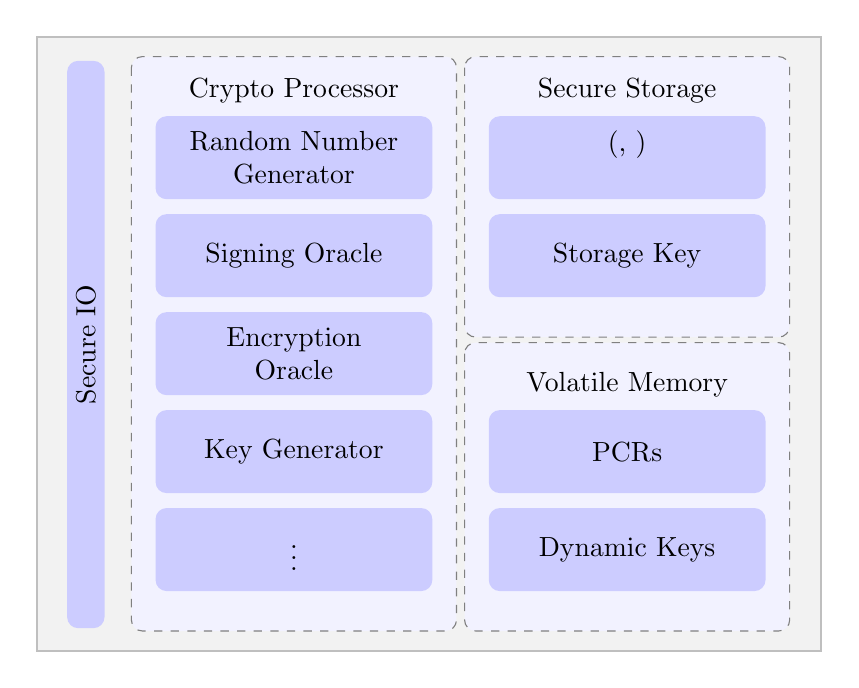
\begin{tikzpicture}
    \node (io) [minimum width=20.5em, fill=blue!20, rounded corners, rotate=90] {Secure IO};
    \node (rng) [minimum width=10em, minimum height=3em, align=center, fill=blue!20, rounded corners, right=2.5em of io, anchor=north west, yshift=-2em] {Random Number \\ Generator};
    \node (sign) [minimum width=10em, minimum height=3em, align=center, fill=blue!20, rounded corners, below=0.5em of rng.south, anchor=north] {Signing Oracle};
    \node (enc) [minimum width=10em, minimum height=3em, align=center, fill=blue!20, rounded corners, below=0.5em of sign.south, anchor=north] {Encryption \\ Oracle};
    \node (gen) [minimum width=10em, minimum height=3em, align=center, fill=blue!20, rounded corners, below=0.5em of enc.south, 
    anchor=north] {Key Generator};
    \node (misc) [minimum width=10em, minimum height=3em, align=center, fill=blue!20, rounded corners, below=0.5em of gen.south, anchor=north] {\vdots};

    \node (ekey) [minimum width=10em, minimum height=3em, align=center, fill=blue!20, rounded corners, right=2em of rng] {(\pktpm, \sktpm) \\ \cert{\ca}{\tpm}};
    \node (skey) [minimum width=10em, minimum height=3em, align=center, fill=blue!20, rounded corners, below = 0.5em of ekey.south] {Storage Key};

    \node (pcr) [minimum width=10em, minimum height=3em, align=center, fill=blue!20, rounded corners, right=2em of gen] {PCRs};
    \node (mkey) [minimum width=10em, minimum height=3em, align=center, fill=blue!20, rounded corners, below = 0.5em of pcr] {Dynamic Keys};

    \node (enclabel) [draw=none, above=0.1em of rng.north] {Crypto Processor};
    \node (storelabel) [draw=none, above=0.1em of ekey.north] {Secure Storage}; 
    \node (memlabel) [draw=none, above=0.1em of pcr.north] {Volatile Memory}; 
    % \node (tpmlabel) [draw=none, above=2.5em of rng.north, xshift=4.5em] {\textbf{Trusted Platform Module}}; 
 
    \begin{pgfonlayer}{background}
        % Compute a few helper coordinates

        \path (rng.north west)+(-1.5,1) node (a) {};
        \path (mkey.south east)+(+0.7,-0.75) node (b) {};
        \path[fill=black!5, draw=gray!50, thick]
            (a) rectangle (b);

        \path (rng.north west)+(-0.3,0.75) node (a) {};
        \path (misc.south east)+(+0.3,-0.5) node (b) {};
        \path[fill=blue!5,rounded corners, draw=black!50, dashed]
            (a) rectangle (b);

        \path (ekey.north west)+(-0.3,0.75) node (c) {};
        \path (skey.south east)+(+0.3,-0.5) node (d) {};
        \path[fill=blue!5,rounded corners, draw=black!50, dashed]
            (c) rectangle (d);     

        \path (pcr.north west)+(-0.3,0.85) node (e) {};
        \path (mkey.south east)+(+0.3,-0.5) node (f) {};
        \path[fill=blue!5,rounded corners, draw=black!50, dashed]
            (e) rectangle (f);            
    \end{pgfonlayer}
\end{tikzpicture}

\caption{\label{fig:tpm} Summary of Trusted Platform Module components. All access to the TPM is mediated by a secure input/output layer to maintain the integrity of protected contents and to ensure that only authorized code can utilize trusted services.}
\end{figure}

One of the main problems to address in realizing trusted computing is establishing a ``root of trust'' on a given system. In the previous lecture, we saw how certificate authorities can be viewed as a root of trust from which other trust relationships are extended. However, to do this we had to assume that the CA's public key is known to any party who verifies a certificate, and that only the CA is able to us its private key to issue certificates. If we want to be able to interact with a remote system, whose hardware we cannot directly inspect, then we need some way of establishing trust in statements made by the system regarding its configuration and software.

One idea is to store a secret key that is unique to the system, perhaps within the operating system. That way, the operating system could inspect the code running on the machine when needed, and sign a corresponding statement with the secret key. However, for others to trust these statements, they would also then need to trust that the operating system itself has not been compromised and had not leaked its signing key. In principle this might seem fine, but in practice this is a rather strong assumption to make because conventional OSes are large, buggy pieces of software that get compromised routinely. 

In short, adding the OS to the \emph{trusted computing base} is a bad idea because it is too large and therefore difficult to account for. Perhaps instead we could push the secret key further down in the platform stack, perhaps in the BIOS or as a priveleged instruction implemented by the CPU itself. To mitigate the risk of leaking the signing key, we can expose a function that uses the key to sign messages (called a \emph{signing oracle}), rather than exposing the key itself. However, typical BIOS functions and priveleged instructions can be invoked by the OS, and since we do not trust the OS, the signing oracle should only be accessible to certain pieces of known, trusted code running on the system.

This is essentially the idea behind the \emph{Trusted Platform Module} (TPM). TPM is a standard for secure hardware co-processors that provide functionality for securely storing of small amounts of data, signing data with trusted keys, and measuring the state of the system (e.g., registers, memory, \ldots). The secure storage on the TPM comes pre-loaded with a unique key pair $(\pktpm, \sktpm)$ as well as a certificate issued by a trusted CA $\cert{\ca}{\tpm} \equiv \sign{\skca}{\iskey{\tpm}{\pktpm}}$. The volatile memory in the TPM is used to store keys that are generated dynamically as software makes requests, as well as a set of \emph{Platform Configuration Registers} that are used to store hash values that reflect the code currently running on the system. Importantly, the TPM is implemented as a tamper-proof hardware component with strong separation from the software running on the system, so the contents of the secure storage remain secret and the contents of volatile memory cannot be modified by rogue software. An overview is shown in Figure~\ref{fig:tpm}.

\subsection{Roots of trust}

The fact that the TPM resides in hardware that cannot be tampered with by software or by physical means establishes a core ``root of trust'' on which TPM-based statements can be based. The architecture of the TPM breaks this down a bit further into several associated roots of trust that cover specific aspects of the TPM's responsibilities, defining the \emph{root of trust for measurement} (RTM) and \emph{root of trust for reporting} (RTR).

\paragraph{Root of trust for measurement.} The RTM addresses the question, \emph{can we trust the component that examined system state reflected in the report}? The RTM must initiate the process of \emph{measuring} the current state of the system, and ensure that it only hands this responsibility off to another trustworthy component. The TPM itself has no visibility into the rest of the system, so this root of trust must necessarily reside outside of the trusted hardware, and it must run before any other untrusted components. If it ran \emph{after} an untrusted component, then there would be no reason to believe that the untrusted component did not violate the integrity of the RTM. 

In practice, one way to establish this root of trust is to place it in the BIOS boot block, which is called the \emph{core} RTM. The BIOS boot block is the first piece of code that runs when a system is started, and it must be trusted to faithfully record a hash of itself and the code that it hands control of the system to after performing its normal functions. In this way, it begins a series of handoffs that can later be inspected to form a transitive chain of trust from the CRTM to the operating system and applications that are eventually loaded and run on the system.

\paragraph{Root of trust for reporting.} The RTM establishes trust in the process responsible for measuring the current state of the system. But in order to create a report for remote principals that attests to the integrity of the system state, these measurements must be stored securely prior to reporting. In particular, once measurements have been taken it should not be possible for software running on the system to overwrite or erase them, as this would allow rogue software like malware to cover its tracks. 

This component is implemented by the TPM, and relies heavily on what are called \emph{Platform Configuration Registers} (PCRs). The TPM has several dozen PCRs, which are 20 bytes in length (the size of a hash), in its volatile memory. However, the PCRs cannot be written to directly by software running on the system. Rather, the only way to update a PCR is to \emph{extend} it, as shown in Equation~\ref{eq:extend}.
\begin{equation}
\label{eq:extend}
\extend{n}{D} \eqdef \pcr[n] \gets H(\pcr[n] \| D)
\end{equation}
In (\ref{eq:extend}), $n$ is the PCR register number, $D$ is a digest (i.e., block of bytes representing current state), and $H$ is a hash function. The state of the specified register is updated with the hash of its current state, concatenated with the given digest. In this way \extend{\cdot} creates a \emph{hash chain} in each register, which can be easily verified by any party who knows the correct sequence of $\pcr[n]$ values, but is difficult to forge as long as $H$ is a good cryptographic hash function.

To understand this in a bit more detail, consider a scenario where the intial value of $\pcr[1]$ was set to 0. Then suppose that it was extended twice, with \extend{1}{D_1} and \extend{1}{D_2}.
\begin{align*}
\text{After}~\extend{1}{D_1},\ \ \  & \pcr[1] = H(D_1) \\
\text{After}~\extend{1}{D_2},\ \ \  & \pcr[1] = H(H(D_1) \| D_2)
\end{align*}
Then if an application reports that the state of the system was $D_1$ followed by $D_2$, one can easily verify this by running the hash function. But if a malicious party wishes instead to report that the state of the system was something else, say $E_1$ followed by $E_2$, then they need to solve for two equations.
\begin{align*}
\text{Find}~E_1~\text{such that}\ \ \  & H(E_1) = H(D_1) \\
\text{Find}~E_2~\text{such that}\ \ \  & H(H(E_1) \| E_2) = H(H(D_1) \| D_2)
\end{align*}
Hash functions for which this problem is computationally infeasible are called \emph{preimage-resistant}, and all cryptographic hash functions satisfy this property.

\section{Measuring system state}

The two roots of trust lay the foundation for the TPM's primary functions, which is to provide trustworthy information that can be used to verify the state of the system. In the context of trusted platforms, this process is called \emph{measurement}. There are two settings in which measurement routinely happens, namely at boot time and then later as needed by user applications.

\subsection{Authenticated boot}

\begin{figure}
\centering

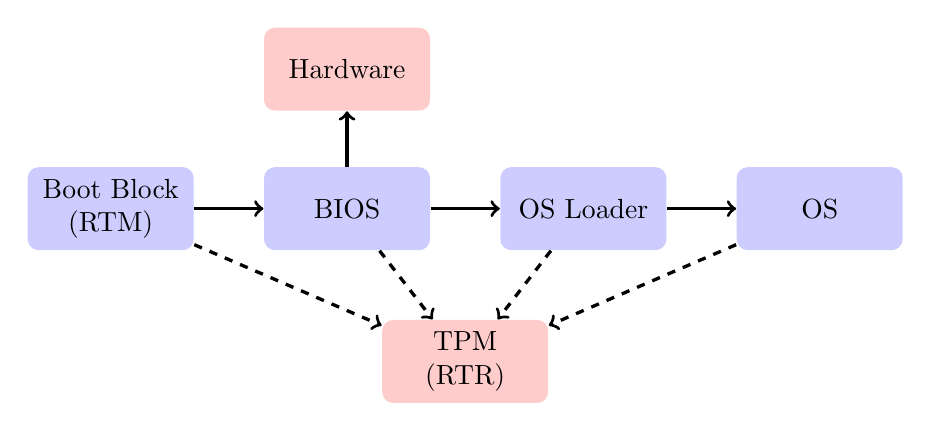
\begin{tikzpicture}
    \node (bootblock) [minimum width=6em, minimum height=3em, align=center, fill=blue!20, rounded corners] {Boot Block \\ (RTM)};
    \node (bios)  [minimum width=6em, minimum height=3em, align=center, fill=blue!20, rounded corners, right=2.5em of bootblock] {BIOS};
    \node (loader)  [minimum width=6em, minimum height=3em, align=center, fill=blue!20, rounded corners, right=2.5em of bios] {OS Loader};
    \node (os)  [minimum width=6em, minimum height=3em, align=center, fill=blue!20, rounded corners, right=2.5em of loader] {OS};
    \coordinate (mid) at ($(bios)!0.5!(loader)$);
    \node (tpm)  [minimum width=6em, minimum height=3em, align=center, fill=red!20, rounded corners, below=4em of mid] {TPM \\ (RTR)};
    \node (hard) [minimum width=6em, minimum height=3em, align=center, fill=red!20, rounded corners, above=2em of bios] {Hardware};

    \draw[very thick,->] (bootblock) -- (bios);
    \draw[very thick,->] (bios) -- (loader);
    \draw[very thick,->] (loader) -- (os);
    \draw[very thick,->] (bios) -- (hard);
    \draw[very thick,dashed,->] (bootblock) -- (tpm);
    \draw[very thick,dashed,->] (bios) -- (tpm);
    \draw[very thick,dashed,->] (loader) -- (tpm);
    \draw[very thick,dashed,->] (os) -- (tpm);
\end{tikzpicture}
\caption{\label{fig:boot} Authenticated boot process. Solid arrows denote measurements, and dashed arrows denote PCR extend operations. The root of trust for measurement is the BIOS boot block, and the root of trust for reporting is the TPM.}
\end{figure}

The fundamental idea behind authenticated boot is to establish that the final software platform, i.e. the operating system and its various components, was correctly loaded into memory and executed as expected by the user or system administrator. To accomplish this, each stage of the system's boot process must be carefully modified to make use of the RTR so that a secure record of each piece of code involved in setting up the system is maintained. This of course starts with the RTM, which records a digest of the next piece of code that runs and extends a PCR with it. Each bit of code continues in this manner, by measuring (i.e., computing a digest of) the \emph{next} piece of code and extending a PCR.

This process is shown in Figure~\ref{fig:boot}, with the typical stages of boot for commodity platforms. Because the BIOS boot block is the root of trust for measurement, it begins the process of measuring the next code to run. At each stage, the root of trust for reporting is utilized by extending the TPM's PCR registers with a digest summary of the next code immediately prior to handoff. When this finishes, one can verify that the code used to boot the system was trustworthy by inspecting the appropriate PCR, and checking its value against the expected digest of each stage's code.

Note that this process ultimately relies on each stage trusting the next to accurately report subsequent measurements. For example, if the BIOS had ``hidden'' functionality that recorded a measurement for malicious code, or even worse if the BIOS reported a measurement for the OS loader and then instead handed control to some malicious code, then the entire process has been subverted. Once the malicious code takes control, then it can extend the PCR with whatever values it chooses, and as long as the RTM remains trusted, then those values will be trusted.

Another important point about this process is that it assumes that whoever verifies the PCR contents is able to determine the suitability of the platform from the digest summaries. However, the digest will only depend on the actual bytes that comprise the code running on the system, and say nothing about the semantics of that code. For example, a trusted party might implement an OS loader that contains vulnerabilities, which as we know can be difficult to identify. So even though the loader is trusted to do the right thing, it may be possible to subvert it while still passing PCR checks, because they say nothing about the behavior of the corresponding code.

\subsection{Application integrity}

Measurement does not need to end with the operating system, as there is no reason that this process shouldn't continue indefinitely as applications are executed on the system. Once it is established that the operating system is trusted, it can measure other applications' code and report the resulting PCR values to interested parties.

\section{Using trusted measurements}

The platform measurement process is the basis for most of the TPM's functionality, and can be used to implement a wide range of secure functionality. We will discuss two of the most important and widely-deployed examples, \emph{remote attestation} and \emph{sealed storage}.

\subsection{Attestation}

Once the system state is measured and recorded in secure PCRs, the process of reporting these measurements to remote systems is called \emph{attestation}. Recall that the TPM has its own unique key pair $(\pktpm,\sktpm)$ and a certificate $\cert{\ca}{\tpm}$ vouching for the authenticity \pktpm. It may seem that attesting to the state of the system at any point is as simple as using \sktpm to sign the contents of specified PCRs, and indeed for some purposes this may be just fine. 
\begin{equation}
\label{eq:pcrval}
\sign{\sktpm}{\pcr[i] = \mathit{GoodHashVal}}
\end{equation}
In particular, when used in combination with the TPM's CA-issued certificate, (\ref{eq:pcrval}) would allow one to conclude that at some point since boot the state of the system was properly configured.

But the usefulness of this fact is rather limited, and many of the applications that trusted platform enables need more. In particular, remote systems often want to verify that they are communicating with an uncompromised host before giving them access to sensitive resources.
\begin{enumerate}
\item Client system completes authenticated boot, storing measurements in TPM's PCRs.
\item User (on client) wishes  to use an application that consumes protected resources on remote server. User's application initiates a connection to the remote server, and sends a signed statement such as (\ref{eq:pcrval}).
\item The remote server checks the signed PCR values and validates \pktpm, in an attempt to establish that the client is in a secure state.
\item If successful, the server gives the client application access to the protected resources.
\end{enumerate}
There are two big problems with this protocol. First of all, suppose that $\mathit{GoodHashVal}$ in (\ref{eq:pcrval}) is a constant value that never changes when the user attempts to use the remote server. In other words, whenever the remote server attempts to validate the user's platform, it always checks the given PCR values against the same pre-defined constant. Then any adversary will know in advance what value the server checks for, and if they can obtain a statement signed by \tpm to that effect then they can trick the server into believing that it is communicating with a secure client.

This is called a \emph{replay attack}, and the protocol as outlined above is vulnerable to it whenever the client sends the server an attestation over an unsecure channel. All that the attacker needs to do is intercept this message once, and they will be able to violate the guarantees of trusted platform in subsequent connections. This attack can be thwarted by having the server reply initially with a \emph{challenge nonce}, or hard-to-predict value that the client must incorporate into its attestation to establish the freshness of the session. This can be done by appending a hash of the PCR value with the nonce value, signed again with the TPM's secret key as shown below.
\begin{center}
\begin{tabular}{ccc}
Client & & Server \\
\tikzmark{m1} & Initiate connection & \tikzmark{m2} \\[1ex]
\tikzmark{m3} & Challenge nonce $R$ & \tikzmark{m4} \\[1ex]
\tikzmark{m11} & \sign{\sktpm}{\pcr[i], H(\pcr[i] \| R)} & \tikzmark{m12} \\[1ex]
\end{tabular}
\begin{tikzpicture}[overlay, remember picture, yshift=2*\baselineskip]
  \draw [thick,->] ([yshift=-1ex]{pic cs:m1}) to ([yshift=-1ex]{pic cs:m2});
  \draw [thick,->] ([yshift=-1ex]{pic cs:m4}) to ([yshift=-1ex]{pic cs:m3});
  \draw [thick,->] ([yshift=-1ex]{pic cs:m11}) to ([yshift=-1ex]{pic cs:m12});
\end{tikzpicture}
\end{center}

However, this protocol is still vulnerable to a \emph{session hijacking} attack. After the client sends the server the signed attestation, the server will believe that any messages that come over the corresponding channel originated on a secure platform. If an attacker inserts themselves in the middle of the client and server, as with a Man-in-the-Middle attack, then they will be able to again fool the server into accepting rogue messages as trusted.

The only way to thwart the session hijacking attack is for the client and server to establish a \emph{shared secret} that is used to encrypt all subsequent communications between the two. This utilizes additional functionality in the TPM, in particular the key generation routines in the cryptographic processor. After attesting with the server's nonce, the client asks the TPM to generate a new public, private key pair $(\pk{C},\sk{C})$, in addition to a certificate $\cert{\tpm}{\pk{C}}$ for the public key. It then sends the public key and cert to the server. The server likewise generates a secret symmetric key $K$, and uses the client's public key to encrypt and send it back. The client can decrypt the shared symmetric, which it uses to encrypt any subsequent messages to the server (and vice versa). The steps after the server's nonce are shown below.
\begin{center}
\begin{tabular}{ccc}
Client & & Server \\
\tikzmark{m7} & \sign{\sktpm}{\pcr[i], H(\pcr[i] \| R)},\pk{C},\cert{\tpm}{\pk{C}} & \tikzmark{m8} \\[1ex]
\tikzmark{m9} & \encr{\pk{C}}{K} & \tikzmark{m10} \\[1ex]
\end{tabular}
\begin{tikzpicture}[overlay, remember picture, yshift=2*\baselineskip]
  \draw [thick,->] ([yshift=-1ex]{pic cs:m7}) to ([yshift=-1ex]{pic cs:m8});
  \draw [thick,->] ([yshift=-1ex]{pic cs:m10}) to ([yshift=-1ex]{pic cs:m9});
\end{tikzpicture}
\end{center}

Before moving on, it is worth noting some limitations of attestation as we have described it. First, while a successful attestation can give the remote party confidence that the correct software is running, it only describes the state of the system at the time that the application was loaded. As discussed previously, the PCR values say nothing about the correctness or behavior of the attested code, and by extension nothing about the state of the system after the measurement was taken. So for example, if the client application falls victim to a code execution vulnerability (e.g., buffer overflow or ROP) after being measured, then any trust that the remote party has in the client is misplaced because the process currently being  executed on the client is not under their control.

Second, if the secret signing key of a TPM is exposed to malicious parties, attestation cannot be trusted. This is because an attacker can use the compromised key to emulate a TPM, signing false PCR values for any attestation request that it wants. 
Keeping the TPM's signing keys secret is a challenging task, as even a seemingly small timing leak can leave them completely exposed to an adversary who has control of the system in question.

\subsection{Protected storage}

Another important application of TPM measurements is protected storage, such as \verb'dm-crypt' (Linux \& BSD) and BitLocker (Windows). When a machine with TPM is first purchased and initialized, the owner can choose to create a \emph{storage root key} (SRK) \sk{\store} that is stored on the TPM and only accessible after providing a user-defined password. The storage root key is then used to encrypt any number of secret keys $K_1, \ldots, K_n$ that are identified by unique \emph{key handles}, which are used to provide \emph{sealed storage} for particular applications on the system. This is accomplished via the $\seal{\cdot}{\cdot}{\cdot}$ function, which takes three arguments as shown in (\ref{eq:seal}).
\begin{equation}
\label{eq:seal}
\seal{\mathit{key~handle}}{\mathit{PCR~values}}{\mathit{data~block}}
\end{equation}
The data block argument can contain up to 256 bytes of data, and is intended to contain an encryption key that is used to protect data for storage. \keywordfont{seal} returns a ``blob'' encrypted with the SRK-protected $K_i$ corresponding to the given handle, which can only be decrypted by the TPM when the PCR values are consistent with those passed to \keywordfont{seal}. This allows a form of secure storage that requires the system to be in a particular configuration before data can be accessed.

The simplest form of sealed storage protects the entire operating system and all installed applications, and is accomplished by sealing the operating system on disk with PCR values that reflect the correct boot block, BIOS, and OS loader. If any of these change, then the PCR values at boot time will not match those with which the OS was sealed, and it will fail to load. Similarly, one can seal an application's code with PCR values that reflect the correct OS kernel, so that the application will only run if the kernel has not been compromised. This can prevent attempts to violate the trusted computing base assumptions of the developers, or to stymie reverse engineering.

More generally, the ability to place constraints on PCR values for data access enables a wide range of policies relevant to secure software. One challenge faced by software that relies on secret encryption keys is, \emph{how to store the keys so that they are not vulnerable to compromise of other parts of the system}? This is relevant, for instance, to secure HTTP servers that are exposed to untrusted network traffic. If the operating system or some other service becomes compromised, then the secret TLS keys can potentially be exfiltrated by the attacker. This could be addressed by having the server utilize sealing, so that the keys can only be decrypted by an unmodified version of the HTTP daemon. Another use could be to validate that certain conditions were met when a piece of data was signed, for example that sensitive patient records were obtained by an uncompromised database server.

\section{Example: Network File Server}

To wrap up, let's consider a more in-depth example of how trusted platform might enable secure functionality in a distributed environment. Suppose that your instructor \matt stores the gradebook for this course on a networked file server situated in some secure location on campus. Because student privacy is paramount, this server implements strict access controls while making very few assumptions about trust. The access control policy itself isn't particularly interesting, and the server daemon will simply attempt to verify from some assumptions (we will get to these in a minute) that it is indeed \matt who requests the gradebook.
\begin{equation}
\label{eq:nfsproof}
\lsequent{\Gamma}{\says{\matt}{\readf{\text{'15316-grades.xlsx'}}}}
\end{equation}
Because requests will always come from remote hosts, the daemon utilizes trusted platform to ensure that the request originates from a university-issued machine, running an up-to-date operating system that has authenticated \matt. So the server has been configured to trust the TPM CA's public key, embodied in policy $Q_1$.
\begin{equation}
Q_1 \equiv \iskey{\ca}{\pk{\ca}}
\end{equation}
Having issued \matt his laptop, the university also knows the public key of his TPM, and has pre-cached its certificate.
\begin{equation}
Q_2 \equiv \sign{\skca}{\iskey{\tpm}{\pktpm}}
\end{equation}
When \matt powers his machine, it performs an authenticated boot and stores the measurements in the TPM's root of trust for reporting. When this completes, the operating system makes use of the TPM's secure random number generator to construct a public/secret key pair $(\pk{\os},\sk{\os})$, and obtains a certificate from the TPM.
\begin{equation}
Q_3 \equiv \sign{\sktpm}{\iskey{\os}{\pk{\os}}}
\end{equation}
Next \matt must authenticate to the operating system by providing his username and password. Because the operating system is known to the university, it is trusted to issue statements on \matt's behalf after he has successfully authenticated. In particular, the university trusts any requests to read files made by the operating system just as though they had been made directly by \matt himself.
\begin{equation}
\label{eq:osdelegate}
Q_4 \equiv \sign{\sk{\os}}{\forall x . (\says{\os}{\readf{x}}) \limply (\says{\matt}{\readf{x}})}
\end{equation}
$Q_4$ in (\ref{eq:osdelegate}) may seem a bit strange at first glance. The operating system is essentially saying that it is allowed to make file requests on behalf of \matt. Why should the server trust the OS to claim authority for itself on behalf of other principals? We will assume that computing services has done its legwork to vet the operating system, and is confident that it would not make such a statement unless \matt had actually authenticated himself to the OS.

Finally, once logged on \matt issues a command to open up the gradebook. At this point, the OS signs a request to read the appropriate file ($Q_5$, and sends it to the networked file server along with the other policies ($Q_3$ and $Q_4$).
\begin{align}
Q_5 \equiv \sign{\sk{\os}}{\readf{\text{'15316-grades.xlsx'}}}
\end{align}

On the other end, the file server has some work to do before it can decide to send the requested file back to the client. First it needs to be convinced that the software running on \matt's computer is free of compromise and up-to-date as expected. It initiates a remote attestation to check that the PCRs initialized by the authenticated boot match expected values, because if this is not the case then none of the vetting and trust placed in the operating system to make requests on \matt's behalf is warranted. Then it needs to verify that the OS's key was actually signed by the TPM, and not some rogue software on \matt's computer.
\begin{equation}
\text{Check}~\verify{\pk{\tpm}}{\sign{\sktpm}{\iskey{\os}{\pk{\os}}}} = \strue
\end{equation}
Having established the integrity of the OS and the authenticity of its public key, it then checks to make sure that the subsequent statements $Q_4,Q_5$ actually came from the operating system and not some rogue software.
\begin{equation}
\text{Check}~\verify{\pk{\os}}{Q_4},\verify{\pk{\os}}{Q_5} = \strue
\end{equation}
If each of these steps is successful, then the file server can be confident that it is speaking to an uncompromised client, to which \matt has authenticated and issued a command to read the gradebook. Finally, it will attempt to prove the judgement in (\ref{eq:nfsproof}), and if successful send back the contents of the file. Constructing this proof is left as an exercise.

\bibliographystyle{abbrv}
\bibliography{bibliography}
\end{document}